\documentclass[prb,preprint]{revtex4-1} 

\usepackage{amsmath}  
\usepackage{amsfonts} 
\usepackage{graphicx} 
\usepackage{gensymb}
\usepackage{enumerate}

\begin{document}

\title{The Faraday Effect and Calculation of the Verdet Constant for a SF-59 Glass Rod}

\author{Frances Yang}
\email{fyang@smith.edu} 

\author{Isabel Lipartito}
\email{iliparti@smith.edu}
\affiliation{Department of Physics, Smith College, Northampton, MA 01063}

\date{\today}

\begin{abstract}
{The Faraday effect is a shift in the polarization of light as it passes through a medium subject to a magnetic field. We observed the Faraday effect in the following experiment. Polarized light from a 650 nm laser was sent through a SF-59 glass rod in a magnetic field produced by a solenoid. 
We then sent the light through a rotatable polarizer and measured intensity of light passing through with a photodiode. 
This allowed us to determine the shift in polarization as the intensity depends on the relative angle of polarization of the polarizer and the light. 
The voltage across a 1 k$\Omega$ resistor in series with the photodiode was measured. We experimentally confirmed the voltage to be proportional to light intensity.
The laser output was modulated so phase-sensitive detection could be used to remove voltage offsets and fluctuations due to variations in room lighting.
The Verdet constant, a wavelength-dependent coefficient which relates the polarization angle rotation to the strength of the magnetic field, characterizes the strength of the Faraday effect for a specific material.  
We determined the Verdet constant for the rod using two experimental methods.
For the first method, we measured the sinusoidal variation in the voltage as a function of polarizer angle for magnetic fields ranging from -10.6 mT to 21.2 mT. From this, we found the magnetic-field dependent phase shift in polarization from which we calculated a Verdet constant of $17.54 \pm 1.12 \mathrm{~rad/T} \cdot \textrm{m}$.
The second method measured fixed the polarizer at an angle of $45\degree$ relative to light polarization when there was no field. This angle was used because it maximizes the change in light intensity, thus voltage, for a given shift in polarization. 
We measured the voltage for fields ranging from $-31.8$ mT to $31.8$ mT and used this to calculate the Verdet constant of $19.9 \pm 1.0 \mathrm{~rad/T} \cdot \textrm{m}$.
Our colleagues performing these experiments found the Verdet constant to be between 19 and 23$\mathrm{~rad/T} \cdot \textrm{m}$ and between 19 and 21$\mathrm{~rad/T} \cdot \textrm{m}$ from using the first and second methods, respectively.  
We address possible causes of the discrepancy between our value from the second method from that of the first method and from the values obtained by our colleagues.}
\end{abstract}

\maketitle 
\section{Aims}
{
\begin{enumerate}[(a)]
\item To demonstrate the Faraday effect: a rotation of the polarization angle of light as it passes through a birefringent material subject to a magnetic field.

\item To demonstrate that the magnitude of rotation of the polarization angle is proportional to the magnitude of the applied magnetic field.

\item{To determine the Verdet constant ($v_c$), the constant of proportionality relating the change in polarization angle $\Delta \phi$ to the applied magnetic field. The relationship between these quantities can be seen in
\begin{equation}
\label{vconst}
\Delta \phi =v_c \hspace{1pt}B L{_{\textrm{sample}}},
\end{equation}
where $L_{\textrm{sample}}$ is the length of the material the light passes through.}
\end{enumerate}

}
\section{Introduction} 

{The Faraday effect, discovered by Michael Faraday in 1845, was the first experimental demonstration of the interrelation of electricity and magnetism.  
It has a strong historical significance and is a benchmark in the development of electromagnetic theory \cite{melissinos}.  
It also is of primary importance in many contemporary research fields in physics.  
For example, the Faraday Effect is currently being used to probe the properties of systems of interacting quantum spins, or spin-liquids.\cite{spin}


The Faraday effect is a magneto-optical phenomenon in which light of a single wavelength traveling through certain materials subject to a magnetic field, experiences a shift in polarization due to the magnetic field, proportional to the magnetic field strength. 
These materials, called birefringent, have different refractive indices for the right and left circular polarizations of light when a magnetic field is applied. 
As light travels through the material, the relative phase angle between the two polarizations changes, causing the overall polarization plane to rotate as it masses through the material \cite{melissinos}.  

As shown in Eq.(\ref{vconst}) , $v_c$ is a constant of proportionality that relates the change in polarization angle to the change in the magnetic field.\cite{expphysics} 
The value of $v_c$ depends on the medium and the wavelength of the light. 
The intensity of the light is passing through a polarizer is given by $I=I_{0}\cos^{2}(\theta)$, where $\theta$ is the difference in angle between the polarization angles of the laser light and the polarizer.  Maximum intensity of light occurs when these angles are the same. 
When a magnetic field is applied to a material the light is propagating through, there will be a shift in the polarization so the intensity will be given by $I=I_{0}*\cos^{2}(\theta+\phi)$ instead.
}

\section{Procedure}
{Polarized light came from a 650 nm laser, driven by a 400 kHZ square wave from a function generator. 
A 15.2 cm long solenoid with 1400 turns and a DC resistance of 1.6 $\Omega$ was the source of our magnetic field. 
The current for the solenoid was provided by a Keithley 2230-30-1 DC Power Supply. Channel 1 and Channel 2 were connected in parallel to provide sufficient current. The calibration of the solenoid was found by measuring the magnetic field at the center of the solenoid for a current of 0 A to 2.25 A in steps of 0.25 A. 
The calibration constant was calculated to be $10.6 \textrm{~mT/A} \pm 0.05 \text{~mT}$. A 10.2 $\pm$ 0.5 cm SF-59 glass rod, was centered inside the solenoid. SF-59 glass is a heavy flint glass of refractive index 1.95 \cite{optics}.  The light is passed through a polarizer and detected by a photodiode, with the setting at 1 k$\Omega$. 
The photodiode outputs a voltage signal proportional to the detected light intensity\cite{teachspin}. A diagram of the experimental setup is shown in Fig.~\ref{setup}.

\begin{figure}
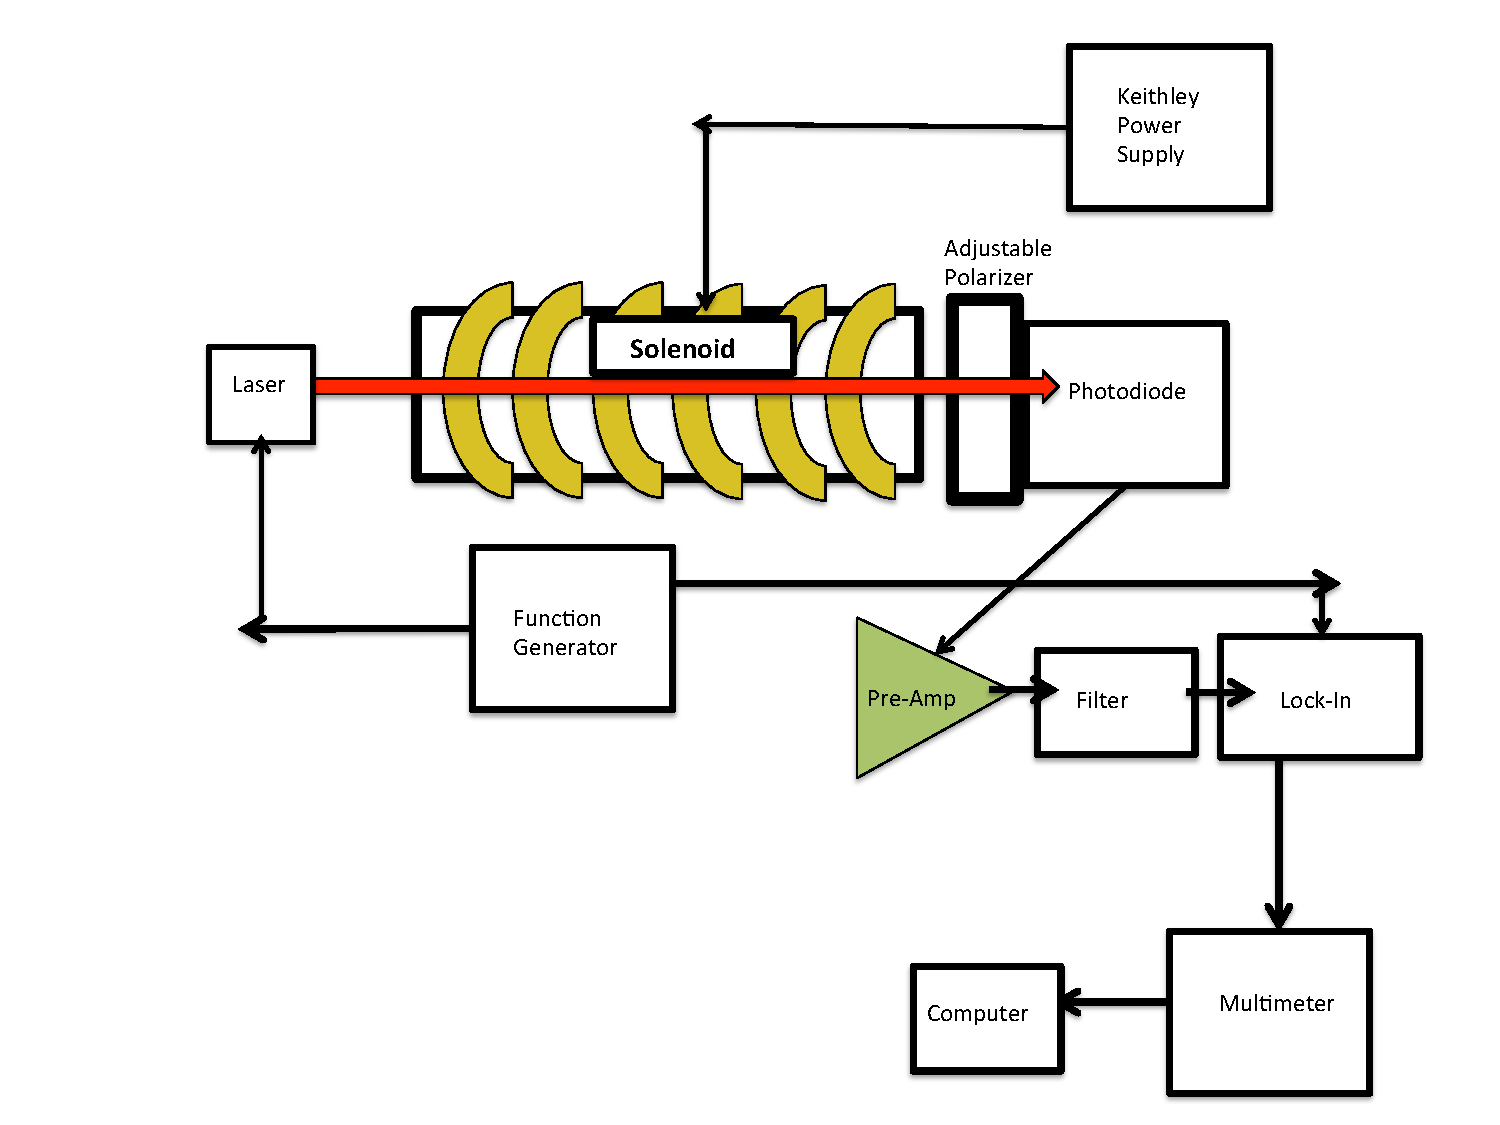
\includegraphics[width = 4.3in]{ExperimentalSetup}
\caption{\label{setup}A flow diagram of our experimental setup}
\end{figure}

A lock-in amplifier was used so undesirable noise such as light from the environment and drift from the photodiode, can be removed from the signal. 
The output of the photodiode was connected to a band pass filter with a center frequency of 400 kHz and a Q of 20. This extracted the first harmonic of the square wave, a 400 kHz sine wave. The output of of the filter was connected to a lock-in amplifier of gain 5. 
The reference signal for the lock-in amplifier was a 400 kHz sine wave with the same phase as the square wave driving the laser. It was generated by the same function generator for the square wave. 
The voltage output signal from the lock-in was measured by a Keithley 2100 Digital Multimeter.

Voltage readings from the multimeter were recorded onto the computer using LabView program (Keithley DC Incremental Write.vi). Each recorded voltage was an average of 16 measurements. We took two types of measurements, so the Verdet constant can be calculated in two ways.  The first method recorded the voltages as the polarizer was rotated in increments of 5\degree. We used this method with magnetic field values of -10.6 mT, 0 mT, 15.9 mT, and 21.2 mT. The negative field was generated by reversing the connection of the two leads of the power supply to the solenoid. The second method set the polarizer at an angle of $\theta = 45\degree$, as it is the angle where we see the largest change in voltage for a small change in polarization. We measured the voltage for fields ranging from $-31.8$ mT to $31.8$ mT, in increments of $5.3$ mT.
}


\section{Results and Analysis}
{\subsection{Method 1: Measurement of Photodiode Voltage for Various Polarizer Angles}
{Figs.~\ref{nofield}--\ref{maxfield} show the measured voltages as a function of the polarizer angle for different magnetic fields. 
The cosine-squared fits we performed are also shown on the plots and the results of the curve fits are listed in Table~\ref{shift table}.

\begin{figure}[h]
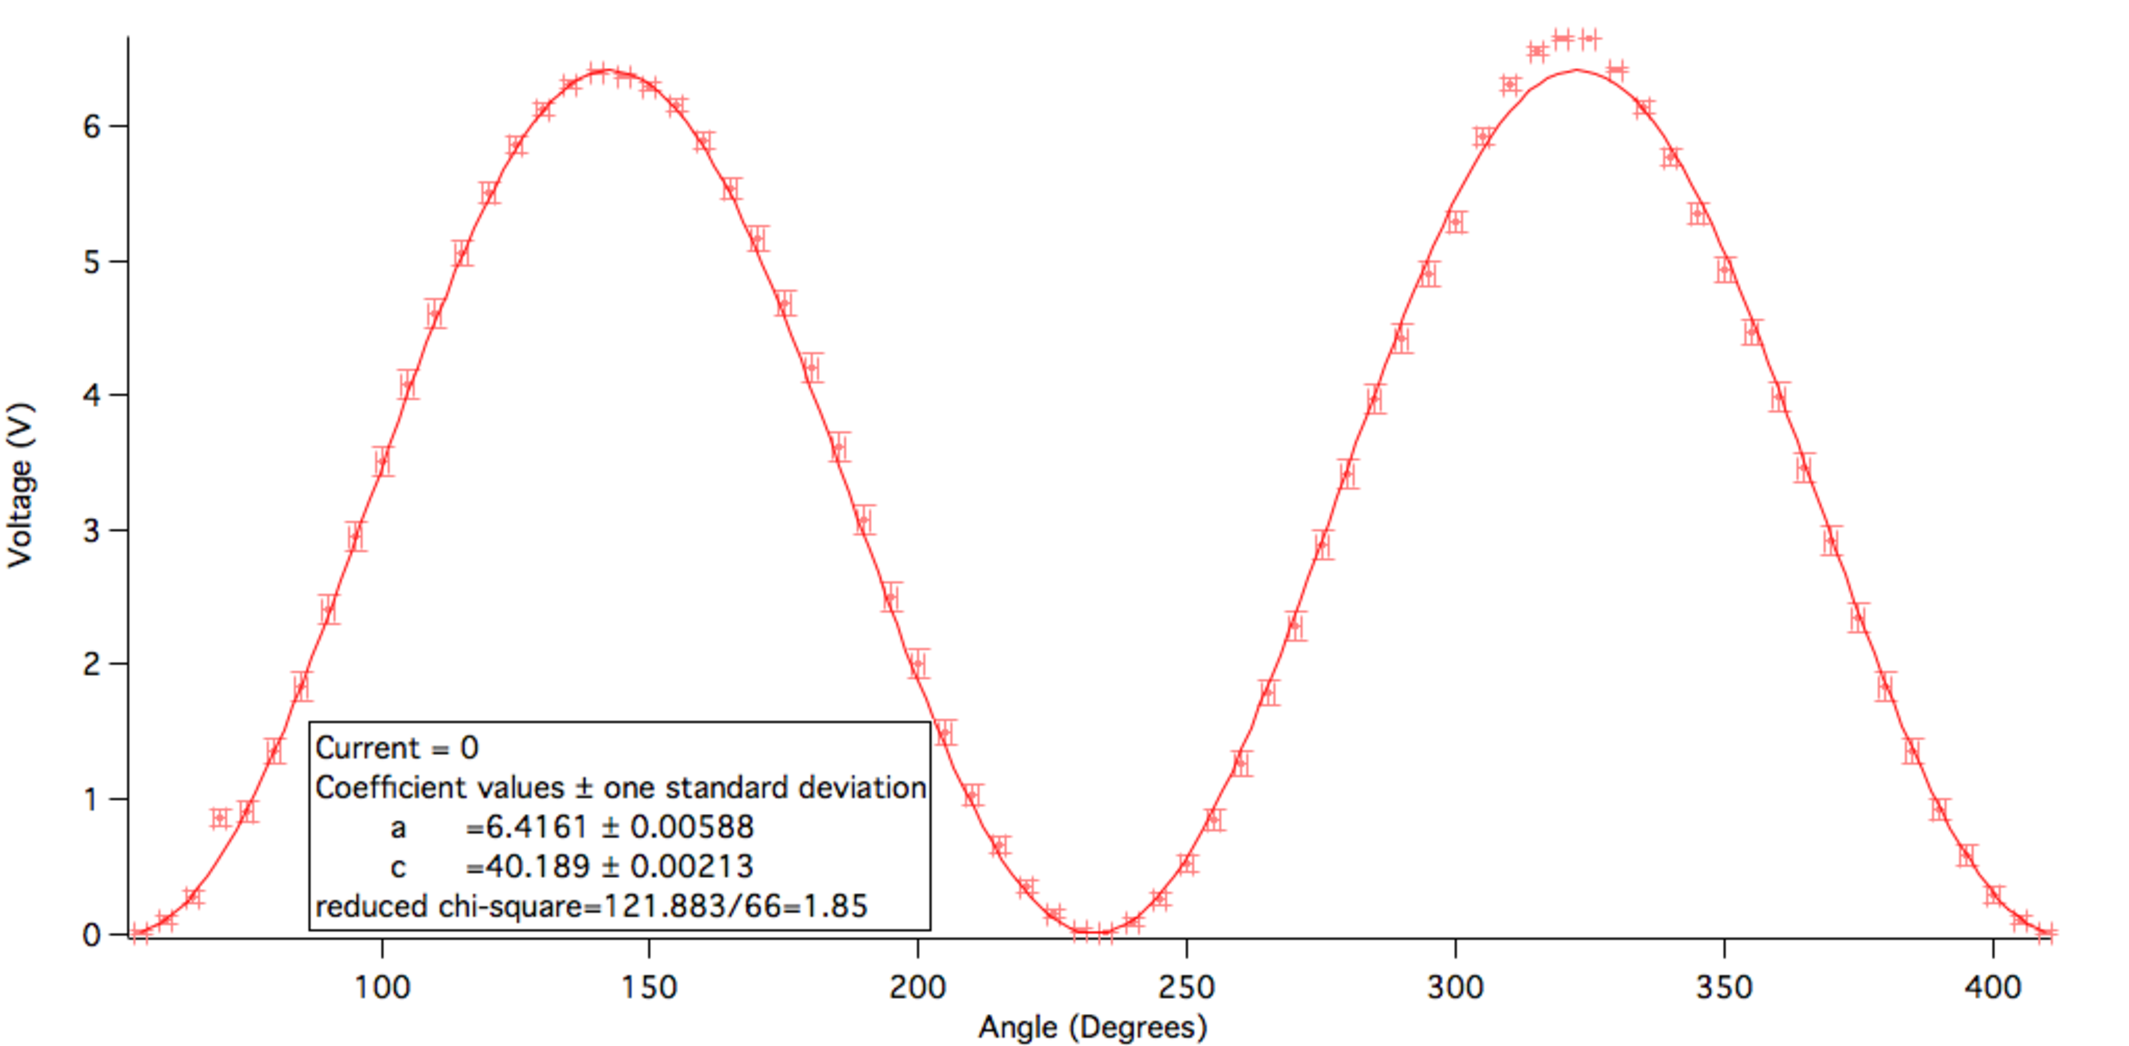
\includegraphics[width = 5.8in]{0A.pdf}
\caption{\label{nofield}Photodiode voltage measured for no magnetic field.}
\end{figure}

One point in the curve fit for the $B=0$ dataset was excluded from the curve fit because we measured the voltage twice for one angle. In all data sets, the experimental measurements of voltage for polarizer angles around $305\degree$--$340\degree$ were systematically higher than the values predicted by the sinusoidal curve fit. 
After a polarizer angle of $340\degree$, we noticed that our experimental data values began to agree once again with the sinusoidal fit.  In the Discussion section, we discuss possible causes for this systematic error. 
We masked the values corresponding to angles of $305\degree$--$340\degree$ from the curve fits as well from datasets with a nonzero magnetic field so they would not skew our calculation of the Verdet constant.
Our dominant source of error in these measurements is from setting the polarizer at the correct angle. We were able to set the polarizer within $1\degree$ of the desired angle. 
This error in the polarizer angle was propagated to an error in the voltage. We neglected voltage reading error from the multimeter as it was many magnitudes smaller than the error due to the angle setting.
We plotted $\Delta \phi$ agains $\Delta B$ in Fig.~\ref{method1pic}. A linear fit was performed to to obtain $\Delta \phi/\Delta B=1.79 \pm 0.07\textrm{~rad/T}$. The Verdet constant was calculated by rearranging Eq.~(\ref{vconst}) to
\begin{equation}
v_c =\frac{1}{L} \frac{\Delta \theta}{\Delta B}. 
\end{equation}
We calculated $v_c$ to be $17.54 \pm 1.12 \mathrm{~rad/T} \cdot \textrm{m}$.
\begin{figure}[h!]
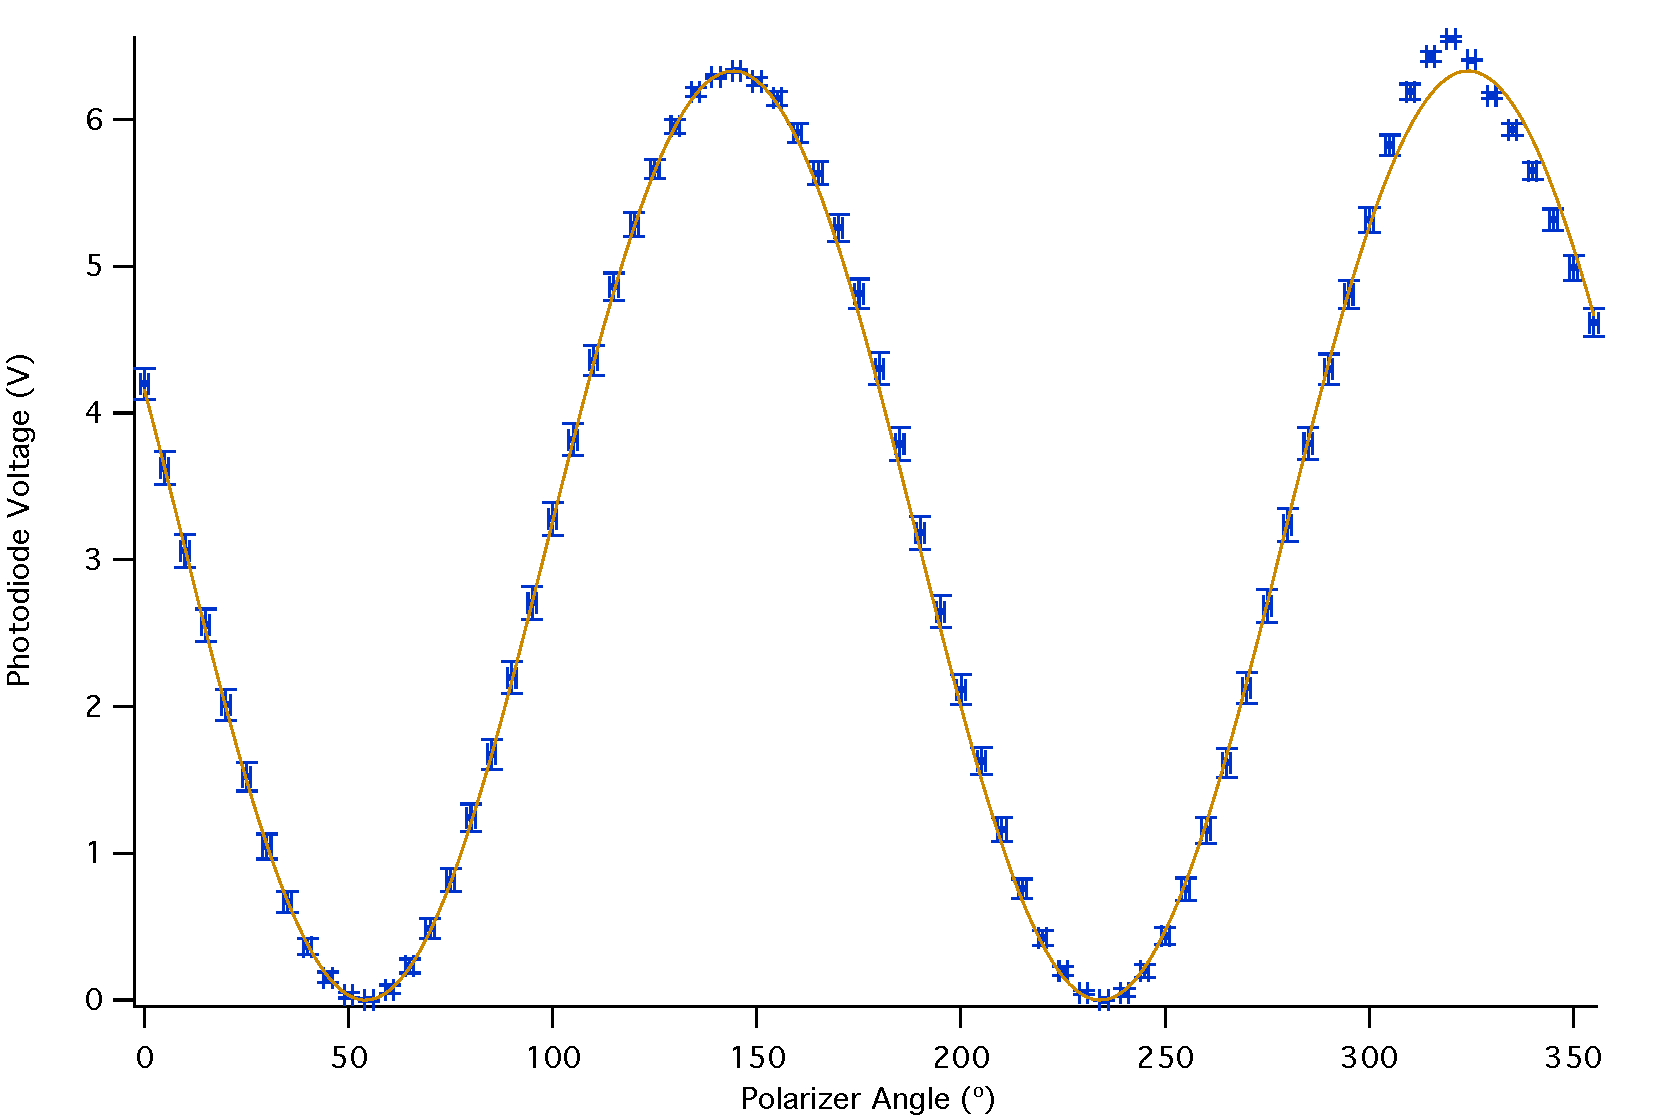
\includegraphics[width = 5.8in]{n1A.pdf}
\caption{\label{neg}Photodiode voltage measured for a magnetic field of -10.6 mT.}
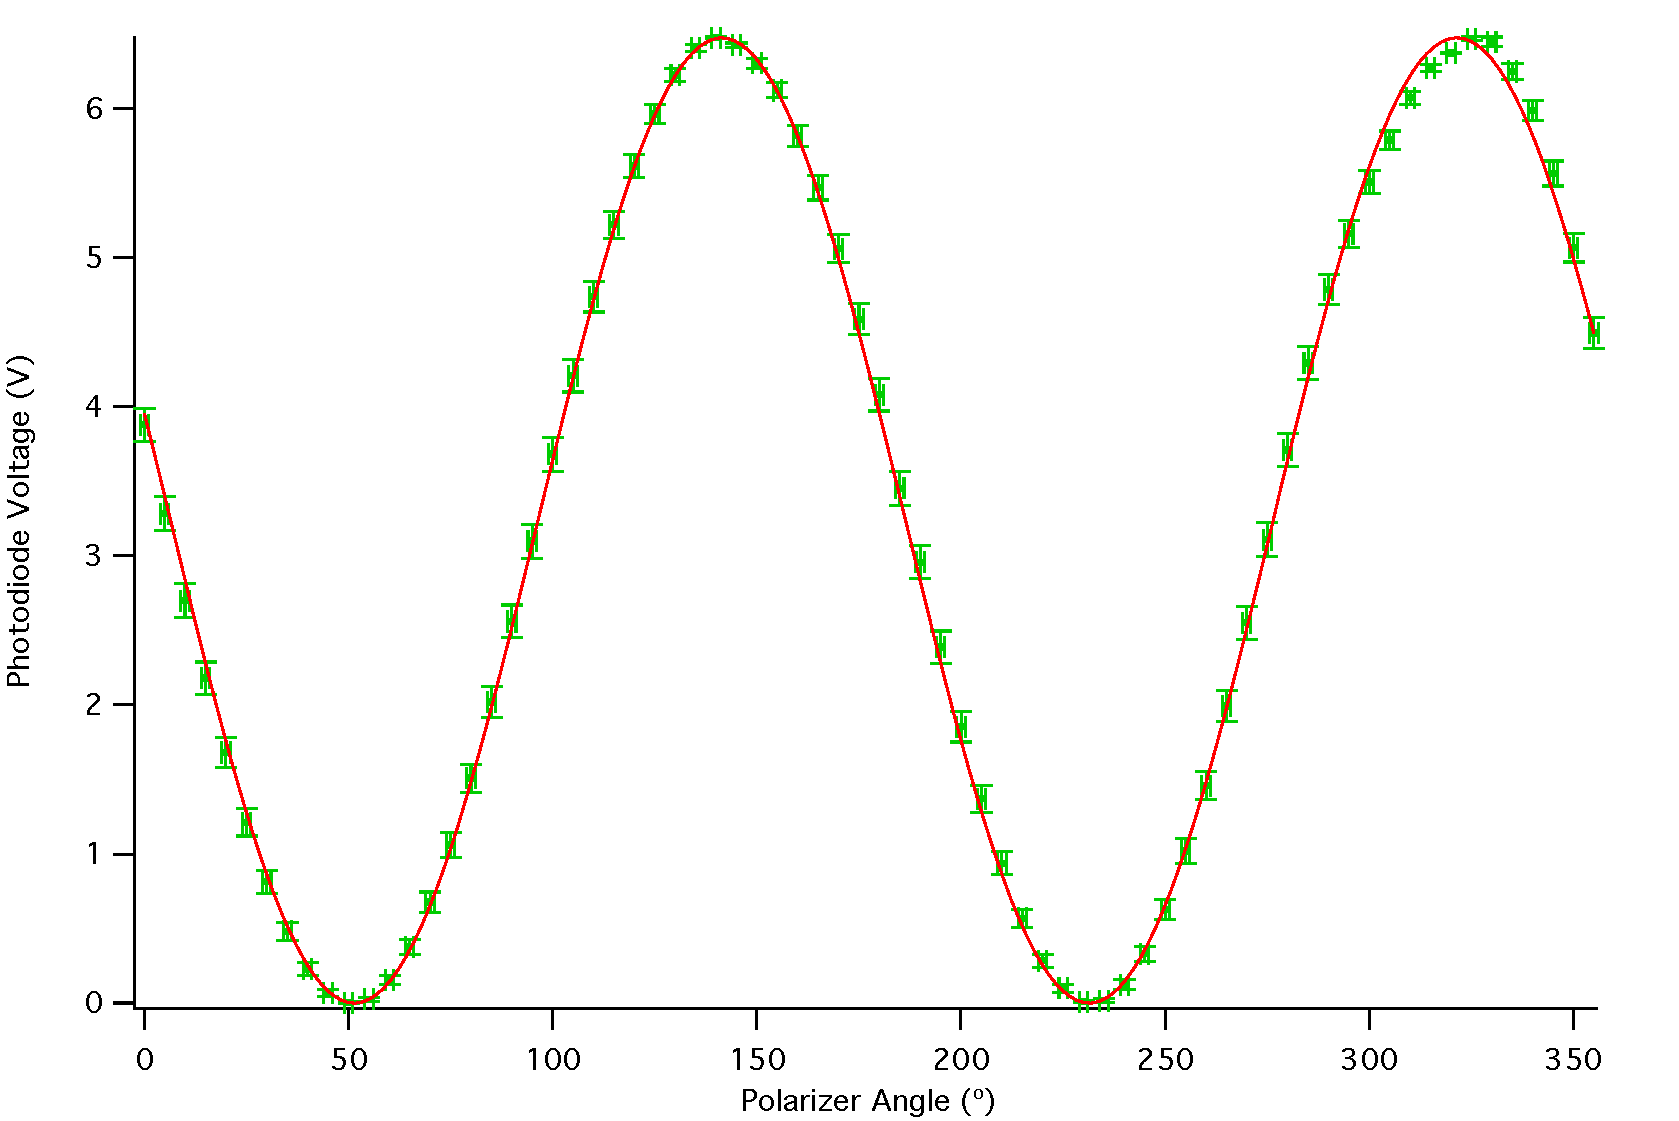
\includegraphics[width = 5.8in]{15A.pdf}
\caption{\label{onehalf}Photodiode voltage measured for a magnetic field of 15.9 mT.}
\end{figure}
\begin{figure}[h!]
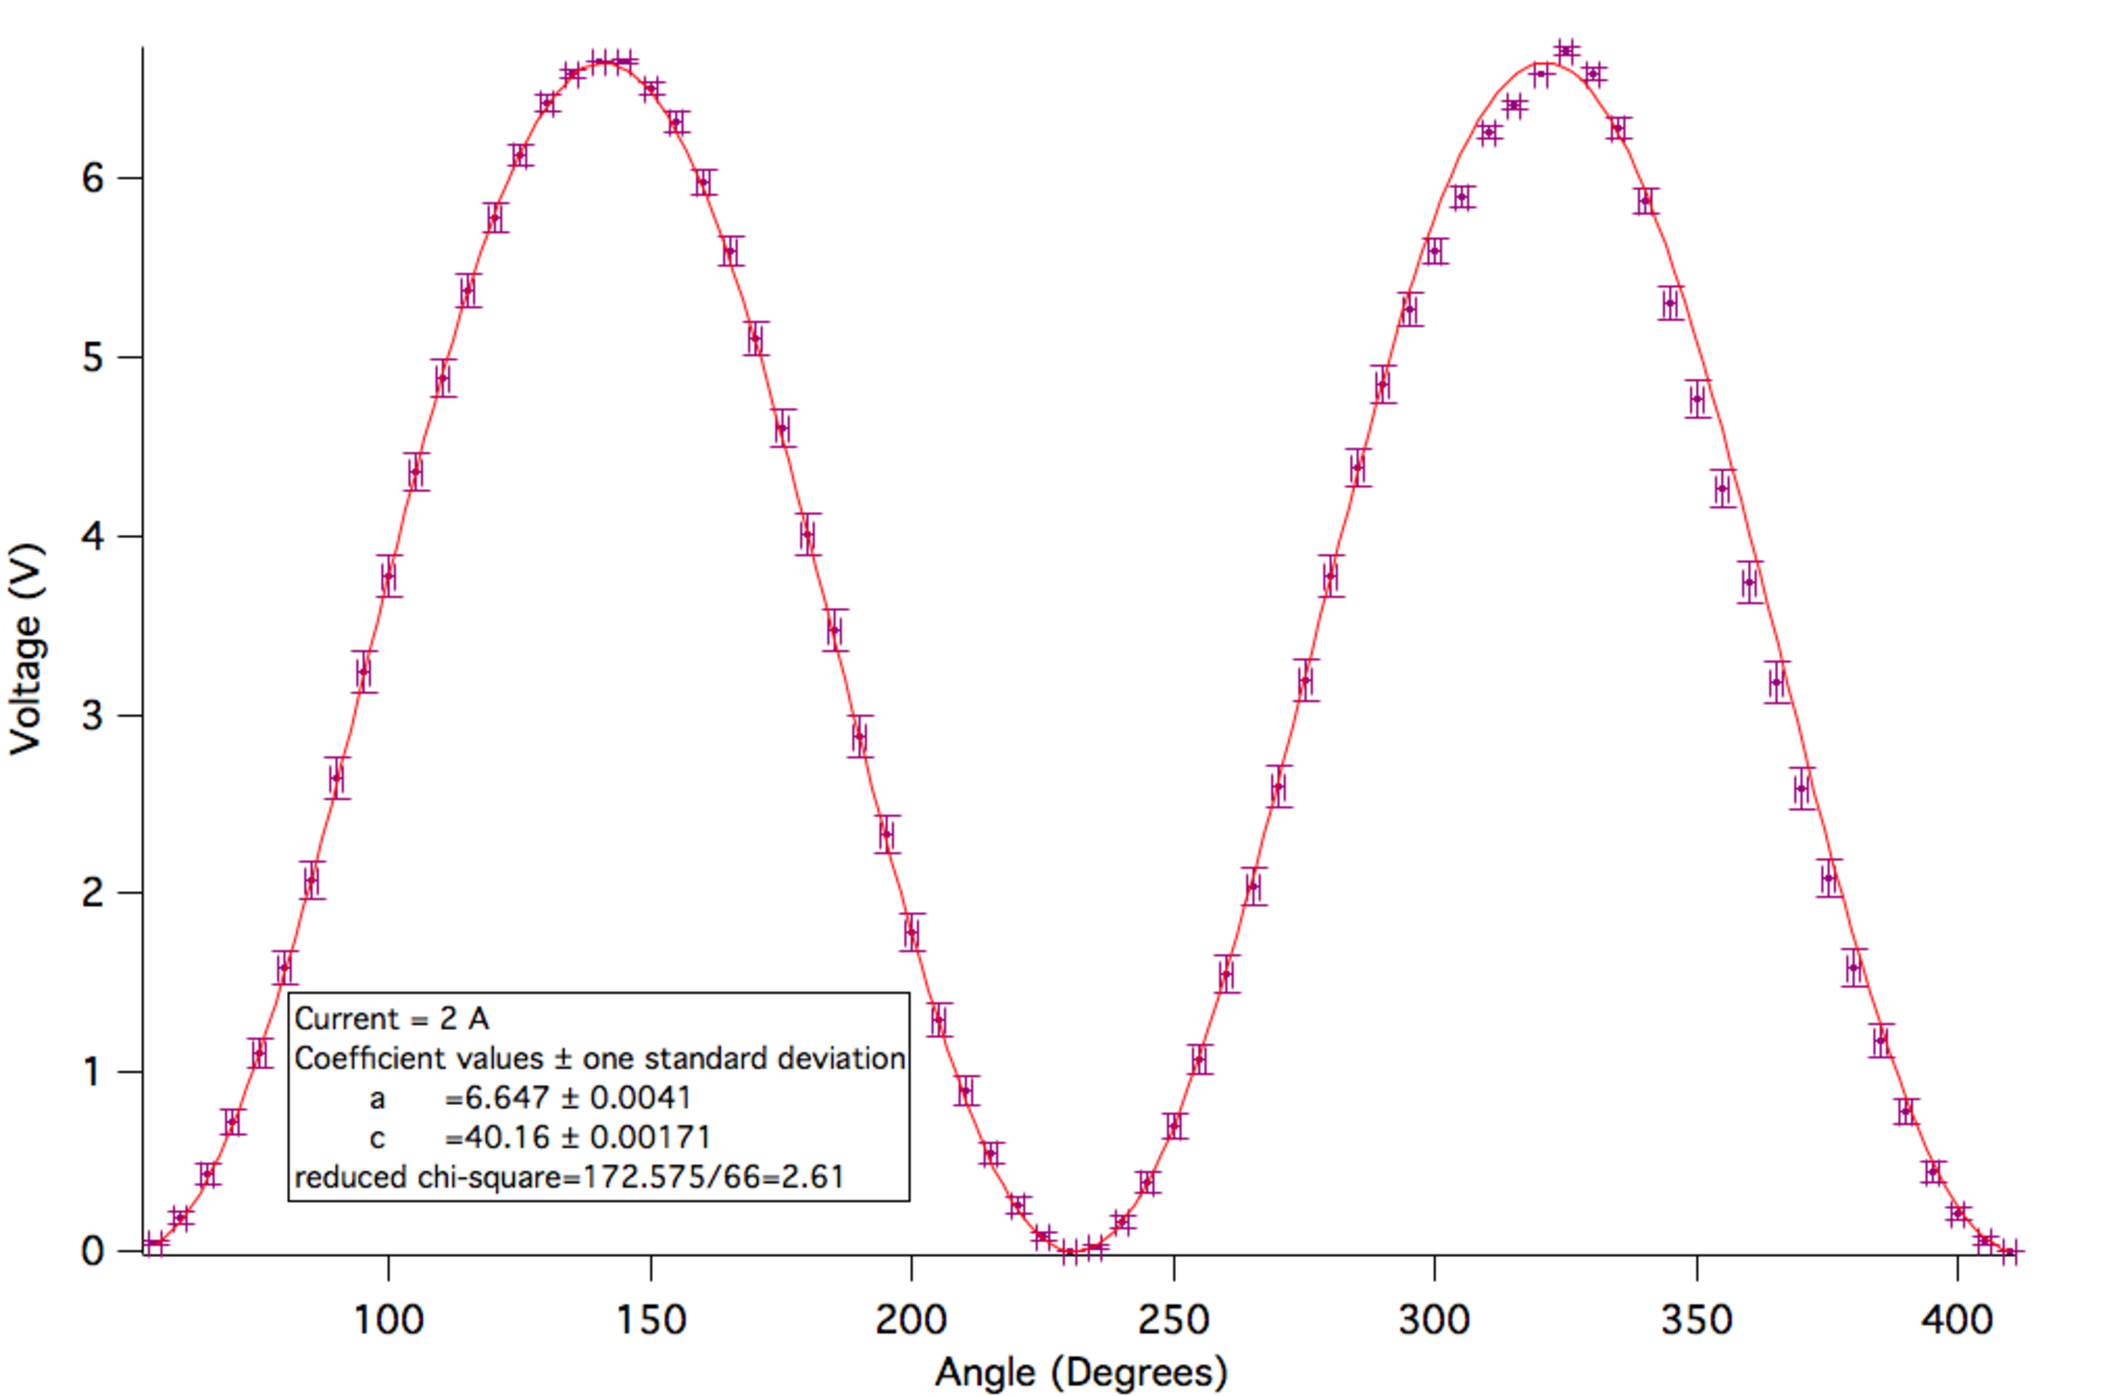
\includegraphics[width = 5.8in]{2A.pdf}
\caption{\label{maxfield}Photodiode voltage measured for a magnetic field of 21.2 mT.}
\end{figure}

\begin{table}
    \begin{ruledtabular}
        \begin{tabular}{ccccc}
            $\Delta$B (mT)&Error $\Delta$B (mT)&$\Delta \phi$ (rad)&Error $\Delta\phi$ ($10^{-5}$ rad)&Reduced $\chi^2$ \\  \hline
            -10.6 & 0.05 & -0.022691 & 187 & 0.76 \\
            0     & 0.05 & -4.77$\cdot10^{-5}$ & 218 & 0.74 \\
            15.9  & 0.05 & 0.024996  & 219 & 0.50 \\
            21.2  & 0.05 & 0.035233  & 184 & 1.17
        \end{tabular}
    \end{ruledtabular}
\caption{\label{shift table}The shift in polarization due to a change in the magnetic field was found from a sinusoidal fit. The reduced $\chi^2$ is a measure of the goodness of fit.}
\end{table}
\begin{figure}
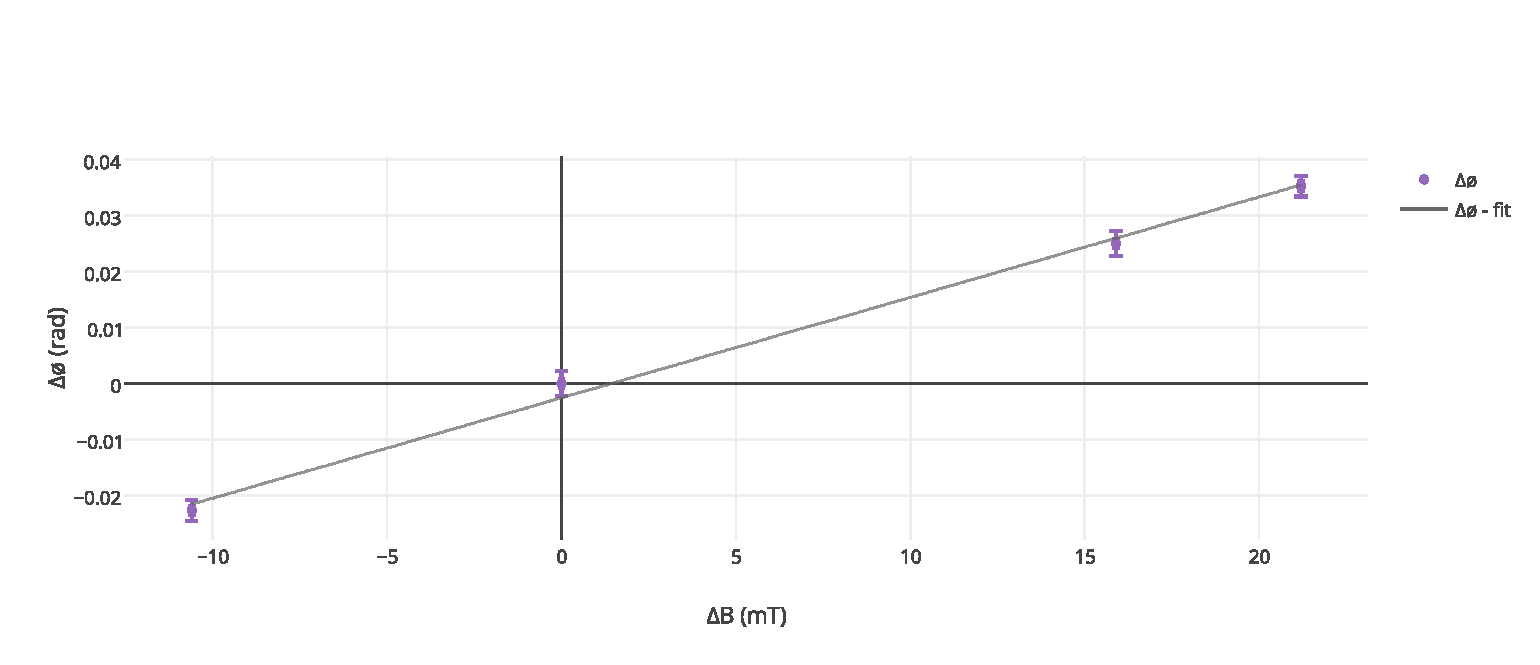
\includegraphics[width =6.3in]{verdet1.pdf}
\caption{\label{method1pic} The relative polarization shift for various magnetic fields. A linear fit was used to determine $\Delta \phi/\Delta B$.}
\end{figure}
}

\newpage
\subsection{Method 2: Measurement of Voltage at $\theta = 45\degree$ for Various B}
{Fig.~\ref{method2pic} shows the voltages measured at an angle of $\theta=45\degree$ for different magnetic fields. 
\begin{figure}
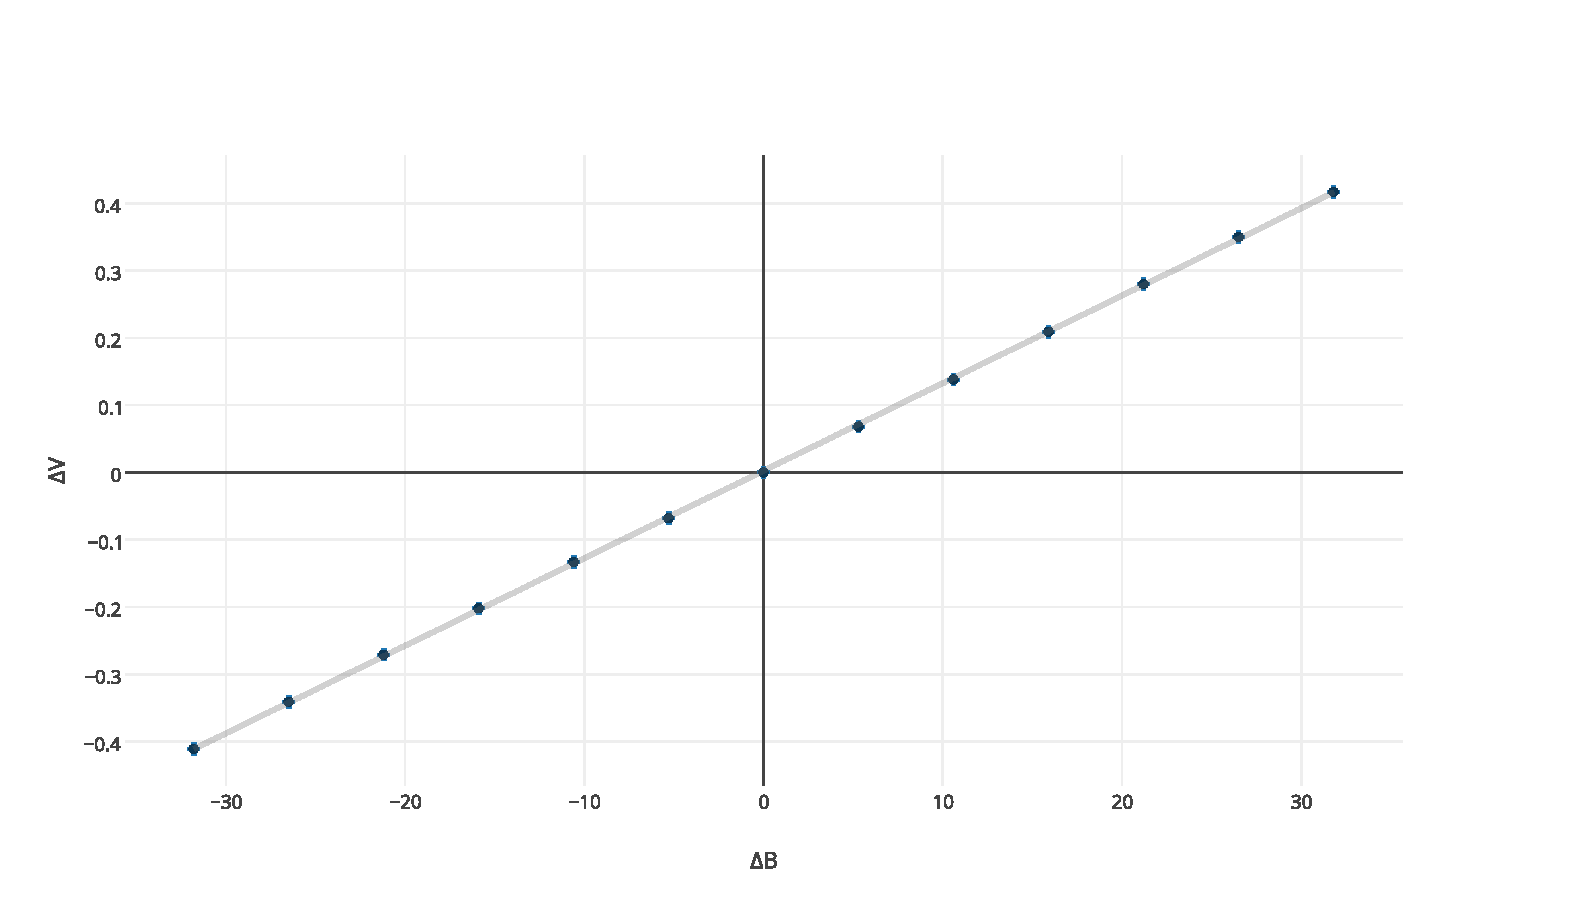
\includegraphics[width =6.3in]{verdetpic2.pdf}
\caption{\label{method2pic} The measured change in photodiode voltage for a change in the magnetic field at a polarizer angle 45\degree\  from the maximum voltage output. A linear fit was used to determine $\Delta V/\Delta B$. The error in our measurements are smaller than the size of our data points.}
\end{figure}
We calculated $v_c$ using 
\begin{equation}
\label{partial}
\left. \frac{\partial V}{\partial B}=\frac{\partial V}{\partial \theta} \frac{\partial \theta}{\partial B}\right|_{\theta=45\degree}.
\end{equation}
Recall that $I=I_{0}\cos^2{\theta}$. Since the voltage from the photodiode is proportional to $I$, $V=V_{0}\cos^2{\theta}$. At $\theta = 45\degree$, $\frac{\partial V}{\partial \theta}=V_0$. 
We performed a linear fit of our data in Fig.~\ref{method1pic} and found $\frac{\partial V}{\partial B}=0.0028\pm 0.0006 \textrm{~V/T}$. We used $V_0=6.405$ V obtained from the curve fit on the data set for no magnetic field. 
The source of error for this method are error in setting the polarizer at $\theta=45\degree$. We believe our error in setting the polarizer angle was one degree, which leads to an error in $\frac{\partial V}{\partial \theta}$ of $0.04\textrm{~V/rad}$. 
We ignored the error in $V_0$ from the curve fit because it was much smaller than the error due to the angle.
From Eq.~(\ref{vconst}) and Eq.~(\ref{partial}), we get
\begin{equation}
\label{2}
v_c =\frac{1}{L}  \frac{\partial V/\partial B}{\partial V/\partial \theta} 
\end{equation}
Using  Eq.~(\ref{2}), we obtained a value of $19.9 \pm 1.0 \mathrm{~rad/T} \cdot \textrm{m}$ for the Verdet constant. }

\section{Discussion}
{Our calculated Verdet constants were $17.54 \pm 1.12 \mathrm{~rad/T} \cdot \textrm{m}$ and $19.9 \pm 1.0 \mathrm{~rad/T} \cdot \textrm{m}$.
The difference between our two calculated values is large enough to be significant. We believe the Verdet constant $19.9 \pm 1.0 \mathrm{~rad/T} \cdot \textrm{m}$ to be closer to the true Verdet constant as our colleagues performing the same experiments found values ranging from 19 to 23 $\mathrm{~rad/T} \cdot \textrm{m}$.
We consider systematic errors present in our data which would have generated an inaccurate value using Method 1.  The most likely parameter which went into Equation 3 that could exhibit a systematic error is our calculation of $\partial \theta/\partial B$. 
 It is possible a systematic error was present in our measurements of the voltage at certain polarizer angles, which led to an error in the phase shift obtained from the sinusoidal fit. We remarked earlier that the $305\degree$--$340\degree$ regions of all four of our datasets were in disagreement with the sinusoidal fit.  
Although we excluded those points from our curve fit, it is possible that measurements at polarizer angles near these were also affected by the same systematic error. The effect was not large enough to be detected by viewing the plots, but could be large enough to affect the sinusoidal fit.
The phase offset was critical for the calculation in Method 1, thus an incorrect offset would give us and incorrect value for the Verdet constant.

We now explore possible causes of this systematic error.  Angle values in the $305\degree$--$340\degree$ range were more difficult to set on the polarizer as they were partially obstructed by the solenoid.  
Using the human eye to set these values and attempting to look beyond the solenoid may have resulted in a systematic error in the angle setting due to parallax.  What looked like $305\degree$ might have actually been $303\degree$--$307\degree$ due to this parallax effect. 
We have also considered the possibility that our polarizer was defective around the problematic values.  
Perhaps the angle markings on the device were improperly applied in the factory and what should have been a certain angle was not actually that angle.  
In order to confirm this, we would need to check the angle settings on the polarizer with a very precise protractor.  


Using Method 2, our colleagues found the $v_c$ to be between 19 and 21$\mathrm{~rad/T} \cdot \textrm{m}$.  Our value, $19.9 \pm 1.0 \mathrm{~rad/T} \cdot \textrm{m}$ is thus in good agreement with the values of our fellow researchers.
Our value for Method 2 did not include the systematic errors we discussed as it did not depend on the sinusoidal fit.  We only needed to set the polarizer to a single angle which itself was out of the problematic angle range.  Our Verdet constant from Method 2 is thus the one to be reported as accurate.  
It was in agreement with the values reported by our colleagues, as mentioned earlier.}

\section{Conclusion}
We used two experimental methods to determine the Verdet constant for a SF-59 glass rod. The two values we found were $17.54 \pm 1.12 \mathrm{~rad/T} \cdot \textrm{m}$ and $19.9 \pm 1.0 \mathrm{~rad/T} \cdot \textrm{m}$. 
The difference between our values is significant. Comparison with the values obtained by our colleagues suggest that there are systematic errors which affected our first experiment, from which we obtained a Verdet constant of $17.54 \pm 1.12 \mathrm{~rad/T} \cdot \textrm{m}$. 
We suspect these systematic errors could be due to improper angle markings on the polarizer at certain angles. They could also be from error in setting the polarizer angle at certain angles due to the way we viewed the apparatus.

To eliminate these systematic errors, we can repeat this experiment with another polarizer to see if there is  still a discrepancy. 
We can also adjust the our viewing angle when we set the polarizer angle. If we look at the polarizer straight on while setting the angle, then we can be accuracy of angle setting would be consistent.
We can improve the precision of our experiment by using a polarizer with finer angle markings so we would be more confident in the setting the polarizer at the correct angle. 
Employing these methods above would allow us probe the significance of the disagreement in our measurements.  
Do they disagree due to the systematic error present in the first method resulting from a possibly defective polarizer, or is their disagreement due to our rather large random errors primarily coming from angle setting? 

To further reduce random errors, we would also want to consider implementing another lock-in amplifier, this one to remove magnetic field noise or fluctuations from sources of magnetic fields other than that from the solenoid.  To expand the scope of this experiment, we could measure the wavelength dependence of the Faraday effect.  In this case, we would repeat our experiments using sources of polarized at different wavelengths. We would repeat our data collection for each of these lasers, and acquire data which could tell us how the strength of the rotation of polarization angle plane depends on different wavelengths of light for a certain value of magnetic field.

One important technological application of the Faraday effect are for optical isolators, which are device that allow the transmission of light in one direction but not the reverse. They are used to protect lasers from being damaged by the back reflection of the light it generates.\cite{optical}
}

\section{References}

\begin{thebibliography}{4}
\bibitem{melissinos} Experiments in Modern Physics.  Adrian Constantin Melissinos and Jim Napolitano.  Gulf Professional Publishing, 2003

\bibitem{teachspin}Instructor's Guide to TeachSpin's FR1-A Apparatus.  Jonathan F. Reichert
\bibitem{spin}Magneto-optical Faraday effect in spin-liquid candidates.  Jacob R. Colbert, H. Dennis Drew, and Patrick A. Lee.  Phys. Rev. B 90, 121105(R) – Published 12 September 2014

\bibitem{expphysics}The Art of Experimental Physics.  Daryn W. Preston and Eric R. Dietz.  John Wiley  $\&$ Sons, Inc, 1991.

\bibitem{optics} The Properties of Optical Glass.  Hans Back and Norbert Neuroth.  Springer Science $\&$ Business Media, 1998.

\bibitem{optical} Visible Free-Space Isolators (395-690 nm).  ThorLabs Product Information Page.  www.thorlabs.com/newgrouppage9.cfm?objectgroupid=2996







\end{thebibliography}


\end{document}
